% AlgoLang 1.0 — presentation (Beamer, XeLaTeX). Build: latexmk -xelatex AlgoLang_Presentation.tex
% By Dr. S. Satyanarayana, Ph.D., PDF (AI) · AlgoProfessor AI R&D Solutions · github.com/drssnaiml1-cell/algolang
\documentclass[aspectratio=169,10pt]{beamer}
\usepackage{fontspec}
\usepackage{tikz}
\usetikzlibrary{arrows.meta,positioning,shapes.geometric,calc,shadows}
\usepackage{booktabs,array,tabularx,colortbl,listings,xcolor}
\usepackage[most]{tcolorbox}

% ─────────── the AlgoLang LaTeX palette (identical to the language manual) ───────────
\definecolor{navy}{HTML}{0B1F3A}
\definecolor{navy2}{HTML}{1D3B66}
\definecolor{navylight}{HTML}{E8EDF5}
\definecolor{gold}{HTML}{C9A227}
\definecolor{goldlight}{HTML}{F3EFE1}
\definecolor{ink}{HTML}{1B1B1B}
\definecolor{muted}{HTML}{5A6270}
\definecolor{rule}{HTML}{D9D4C3}
\definecolor{okgreen}{HTML}{2F6B3A}
\definecolor{badred}{HTML}{7A1020}
\definecolor{codebg}{HTML}{F7F6F1}
\definecolor{termbg}{HTML}{0E1A2B}
\definecolor{termfg}{HTML}{E6E9EF}

\setsansfont{Inter}[BoldFont={Inter SemiBold},Scale=0.94]
\setmonofont{DejaVu Sans Mono}[Scale=0.82]
\newfontfamily\symfont{DejaVu Sans}
\newcommand{\yes}{{\symfont\textcolor{okgreen}{✓}}}
\newcommand{\partly}{{\symfont\textcolor{gold!85!black}{◐}}}
\newcommand{\no}{{\symfont\textcolor{badred}{✗}}}

% ─────────── theme ───────────
\setbeamertemplate{navigation symbols}{}
\setbeamercolor{normal text}{fg=ink,bg=white}
\setbeamercolor{structure}{fg=navy}
\setbeamercolor{frametitle}{fg=white,bg=navy}
\setbeamercolor{alerted text}{fg=gold!85!black}
\setbeamerfont{frametitle}{size=\Large,series=\bfseries}
\setbeamertemplate{itemize item}{\textcolor{gold}{\rule[0.25ex]{0.9ex}{0.9ex}}}
\setbeamertemplate{itemize subitem}{\textcolor{navy2}{\textbullet}}
\setbeamertemplate{frametitle}{%
  \nointerlineskip
  \begin{beamercolorbox}[wd=\paperwidth,ht=2.4em,dp=0.9em,leftskip=1.2em]{frametitle}
    \usebeamerfont{frametitle}\insertframetitle
    \ifx\insertframesubtitle\@empty\else\\[-0.1em]{\small\color{gold}\insertframesubtitle}\fi
  \end{beamercolorbox}%
  \nointerlineskip{\color{gold}\rule{\paperwidth}{2pt}}%
}
\setbeamertemplate{footline}{%
  \leavevmode\hbox{\begin{beamercolorbox}[wd=\paperwidth,ht=2.4ex,dp=1.1ex,leftskip=1.2em,rightskip=1.2em]{normal text}%
    \color{muted}\tiny AlgoLang 1.0 \enspace·\enspace Dr.\ S.\ Satyanarayana, Ph.D., PDF (AI) \enspace·\enspace
    AlgoProfessor AI R\&D Solutions\hfill github.com/drssnaiml1-cell/algolang\enspace\textcolor{gold}{\insertframenumber}
  \end{beamercolorbox}}}

\lstdefinelanguage{AlgoLang}{
  morekeywords={agent,flow,model,tool,par,for,in,if,else,emit,true,false,eval,case,expect,stream,circuit,risk,disclose,untrusted,and,or,contains,not,type,use,as},
  morekeywords=[2]{role,goal,uses,policy},
  morekeywords=[3]{budget,tokens,retry,timeout,require,human,when,confidence,forbid,samples,explain,with,evidence,redact,pii,approvals,always,fair,across,robust,consistency,qpu,shots},
  morekeywords=[4]{text,score,list,json,bool,number,uncertain},
  sensitive=true, morecomment=[l]{//}, morestring=[b]"}
\lstset{basicstyle=\ttfamily\footnotesize\color{ink},keywordstyle=\bfseries\color{navy},
  keywordstyle=[2]\bfseries\color{navy2},keywordstyle=[3]\bfseries\color{gold!75!black},
  keywordstyle=[4]\itshape\color{navy2},commentstyle=\itshape\color{muted},stringstyle=\color{okgreen},
  showstringspaces=false,columns=fullflexible,keepspaces=true,backgroundcolor=\color{codebg},
  frame=leftline,framerule=2.5pt,rulecolor=\color{gold},xleftmargin=6pt,framexleftmargin=4pt,
  aboveskip=2pt,belowskip=2pt,upquote=true}
\lstdefinestyle{py}{language=Python,keywordstyle=\bfseries\color{navy}}

\newcommand{\goldbox}[2]{\begin{tikzpicture}\node[draw=gold,line width=1pt,fill=goldlight,rounded corners=4pt,
  inner sep=7pt,text width=#1,align=left]{#2};\end{tikzpicture}}
\newcommand{\navybox}[2]{\begin{tikzpicture}\node[fill=navy,rounded corners=4pt,inner sep=7pt,text width=#1,
  align=left,text=white]{#2};\end{tikzpicture}}
\newcommand{\stat}[2]{\begin{tikzpicture}\node[draw=gold,line width=1pt,rounded corners=5pt,fill=white,minimum width=2.45cm,
  minimum height=1.5cm,align=center]{{\LARGE\bfseries\color{navy}#1}\\[1pt]{\scriptsize\color{muted}#2}};\end{tikzpicture}}
\tcbset{appcard/.style={enhanced,colback=white,colframe=navy!25,boxrule=0.8pt,arc=4pt,
  left=7pt,right=7pt,top=5pt,bottom=5pt,before skip=0pt,after skip=0pt,before upper=\raggedright}}
\newcommand{\riskpill}[2]{\tikz[baseline=(p.base)]\node[fill=#1,rounded corners=4pt,inner sep=2.2pt,
  text=white,font=\fontsize{6}{7}\selectfont\bfseries](p){#2};}
\newcommand{\govbox}[1]{\tikz\node[fill=goldlight,rounded corners=3pt,inner sep=4pt,text width=\dimexpr\linewidth-8pt\relax,
  align=left,font=\tiny\bfseries,text=navy]{\textcolor{gold!85!black}{■}\enspace #1};}
\renewcommand{\arraystretch}{1.12}
\newcolumntype{L}[1]{>{\raggedright\arraybackslash}p{#1}}
\newcolumntype{Y}{>{\raggedright\arraybackslash}X}

\title{AlgoLang 1.0}
\subtitle{The agent-native programming language for trustworthy AI}
\author{Dr.\ S.\ Satyanarayana, Ph.D., PDF (AI)}
\date{November 2026}

\begin{document}

% ═════════════════════════════ 1 · Title ═════════════════════════════
{\setbeamertemplate{footline}{}
\begin{frame}[plain]

\begin{tikzpicture}[remember picture,overlay]
  \fill[navy] (current page.south west) rectangle (current page.north east);
  \fill[gold] ([yshift=-2.1cm]current page.north west) rectangle ([yshift=-2.18cm]current page.north east);
  \begin{scope}[shift={([xshift=-3.2cm,yshift=0.5cm]current page.east)}]
    \foreach \a in {0,45,...,315} {
      \draw[gold,line width=3pt,line cap=round] (\a:0.55) -- (\a:1.35);
      \fill[gold!90!white] (\a:1.35) circle (0.2);}
    \fill[navy] (0,0) circle (0.5); \fill[gold] (0,0) circle (0.24);
  \end{scope}
  \node[anchor=north west,text=gold,font=\small\bfseries] at ([xshift=1.2cm,yshift=-1.2cm]current page.north west)
    {ALGOPROFESSOR AI R\&D SOLUTIONS · HYDERABAD};
  \node[anchor=west,text=white,font=\fontsize{44}{48}\selectfont\bfseries] at ([xshift=1.2cm,yshift=1.55cm]current page.west)
    {Algo\textcolor{gold}{Lang} 1.0};
  \node[anchor=west,text=white,font=\Large,text width=10cm] at ([xshift=1.2cm,yshift=0.05cm]current page.west)
    {The agent-native programming language\\ for \textcolor{gold}{trustworthy AI}};
  \node[anchor=south west,text=white,font=\large\bfseries] at ([xshift=1.2cm,yshift=2.0cm]current page.south west)
    {Dr.\ S.\ Satyanarayana, Ph.D., PDF (AI)};
  \node[anchor=south west,text=navylight,font=\small] at ([xshift=1.2cm,yshift=1.4cm]current page.south west)
    {Founder, CEO \& Chief Agentic AI Scientist · AlgoProfessor AI R\&D Solutions · www.algoprofessor.com};
  \node[anchor=south west,text=gold,font=\small\ttfamily] at ([xshift=1.2cm,yshift=0.8cm]current page.south west)
    {github.com/drssnaiml1-cell/algolang \quad·\quad Apache 2.0 \quad·\quad November 2026};
\end{tikzpicture}
\end{frame}}

% ═════════════════════════════ 2 · Agenda ═════════════════════════════
\begin{frame}{Agenda}
\begin{columns}[T]
\column{0.48\textwidth}
\begin{enumerate}\setlength\itemsep{3pt}
\item[\textcolor{gold}{\bfseries 01}] The problem: AI decisions nobody can check
\item[\textcolor{gold}{\bfseries 02}] What AlgoLang is, and its design principles
\item[\textcolor{gold}{\bfseries 03}] The language: agents, flows, policies, types
\item[\textcolor{gold}{\bfseries 04}] Compiler, runtime and the AlgoVM
\item[\textcolor{gold}{\bfseries 05}] Governance and Trustworthy AI
\item[\textcolor{gold}{\bfseries 06}] Uncertainty, evals and evidence
\end{enumerate}
\column{0.48\textwidth}
\begin{enumerate}\setlength\itemsep{3pt}
\item[\textcolor{gold}{\bfseries 07}] Real-time events, Quantum AI, interoperability
\item[\textcolor{gold}{\bfseries 08}] Comparison with programming languages
\item[\textcolor{gold}{\bfseries 09}] Comparison with agent frameworks
\item[\textcolor{gold}{\bfseries 10}] 22 enterprise applications
\item[\textcolor{gold}{\bfseries 11}] Toolchain, roadmap, getting started
\item[\textcolor{gold}{\bfseries 12}] Where AlgoLang fits, and collaboration
\end{enumerate}
\end{columns}
\end{frame}

% ═════════════════════════════ 3 · Problem ═════════════════════════════
\begin{frame}{The problem}{AI agents now make decisions that matter, and nobody can check them}
\begin{columns}[T]
\column{0.55\textwidth}
\begin{itemize}\setlength\itemsep{6pt}
\item Loans, triage, claims, admissions and trades are increasingly decided by \alert{LLM agents}.
\item In today's code an agent is just a function call buried in Python: \textbf{no policy, no budget, no reviewer, no record}.
\item Regulation now asks for risk classes, human oversight, transparency and logs (e.g.\ the EU AI Act, India's DPDP Act).
\item Teams bolt these on afterwards, inconsistently, and often not at all.
\end{itemize}
\column{0.42\textwidth}
\goldbox{5.6cm}{\textbf{\color{navy}Four questions every AI decision should answer}\\[4pt]
\textcolor{gold}{1.} Who was allowed to decide?\\
\textcolor{gold}{2.} Why was this the decision?\\
\textcolor{gold}{3.} Was it fair and robust?\\
\textcolor{gold}{4.} Can an auditor prove what happened?\\[4pt]
{\small\color{muted}AlgoLang makes the compiler and runtime answer them, every time.}}
\end{columns}
\end{frame}

% ═════════════════════════════ 4 · What ═════════════════════════════
\begin{frame}{What is AlgoLang?}
\begin{center}
\navybox{12.6cm}{\centering\large AlgoLang is a programming language with \textcolor{gold}{\bfseries no functions}.\\
Every unit of work is an \textcolor{gold}{\bfseries agent} with a role, a goal, explicit tools, a model and a policy.}
\end{center}
\vspace{4pt}
\begin{columns}[T]
\column{0.32\textwidth}\goldbox{3.9cm}{\textbf{\color{navy}Agent}\\[2pt]\small role · goal · tools · model · policy; returns text, score, list, a typed message, or \texttt{uncertain<T>}}
\column{0.32\textwidth}\goldbox{3.9cm}{\textbf{\color{navy}Flow}\\[2pt]\small the only other construct: call agents, run them in parallel, branch, emit results}
\column{0.32\textwidth}\goldbox{3.9cm}{\textbf{\color{navy}Guarantees}\\[2pt]\small policies, budgets, human review and a signed audit log enforced by compiler and runtime}
\end{columns}
\vspace{6pt}
{\small\color{muted}Designed by Dr.\ S.\ Satyanarayana at AlgoProfessor AI R\&D Solutions, Hyderabad. Open source (Apache 2.0).}
\end{frame}

% ═════════════════════════════ 5 · Principles ═════════════════════════════
\begin{frame}{Design principles}
\begin{columns}[T]
\column{0.5\textwidth}
\begin{itemize}\setlength\itemsep{5pt}
\item \textbf{Agents, not functions.} The unit of computation is an accountable agent.
\item \textbf{Policies are code.} Budgets, forbidden attributes and reviewers are declared, and checked before anything runs.
\item \textbf{Uncertainty is a type.} \texttt{uncertain<score>} samples several times and carries its confidence.
\item \textbf{Deterministic guards.} Branch on tool verdicts, not model moods.
\end{itemize}
\column{0.5\textwidth}
\begin{itemize}\setlength\itemsep{5pt}
\item \textbf{People stay in charge.} \texttt{require human}, four-eyes approvals, escalation queues.
\item \textbf{Evidence by default.} A hash-chained, signed audit record for every call.
\item \textbf{Tested like software.} Evals for quality, fairness and robustness in CI.
\item \textbf{Offline first.} A deterministic mock model, so every program runs and tests without an API key.
\end{itemize}
\end{columns}
\end{frame}

% ═════════════════════════════ 6 · Code ═════════════════════════════
\begin{frame}[fragile]{The language at a glance}{A governed loan decision in 20 lines}
\begin{columns}[T]
\column{0.6\textwidth}
\begin{lstlisting}[language=AlgoLang]
risk high "Retail credit decisions"
disclose "An AI system assisted this decision."

agent Affordability(app: text) -> score {
    goal   "Debt-to-income ratio for {app}"
    uses   bureau.pull
    policy { budget tokens 2000  redact pii }
}
agent Committee(app: text, dti: score) -> uncertain<score> {
    goal   "Recommend approval for {app}"
    policy { samples 5  require approvals 2
             forbid gender, religion  explain with evidence }
}
flow main(app: text) {
    dti = Affordability(app)
    if dti > 0.5 { emit Decline(app, dti) }
    else         { emit Committee(app, dti) }
}
\end{lstlisting}
\column{0.37\textwidth}
\small
\begin{itemize}\setlength\itemsep{4pt}
\item \texttt{risk high}: the compiler demands oversight, fairness tests, PII redaction and signed audit.
\item \texttt{budget}, \texttt{forbid}: refused at compile time if violated.
\item \texttt{uncertain<score>}: 5 samples, mean and confidence.
\item \texttt{require approvals 2}: four-eyes review before release.
\item Every call → signed, hash-chained audit.
\end{itemize}
\end{columns}
\end{frame}

% ═════════════════════════════ 7 · Pipeline ═════════════════════════════
\begin{frame}{Compiler and runtime}{From source to governed execution}
\centering
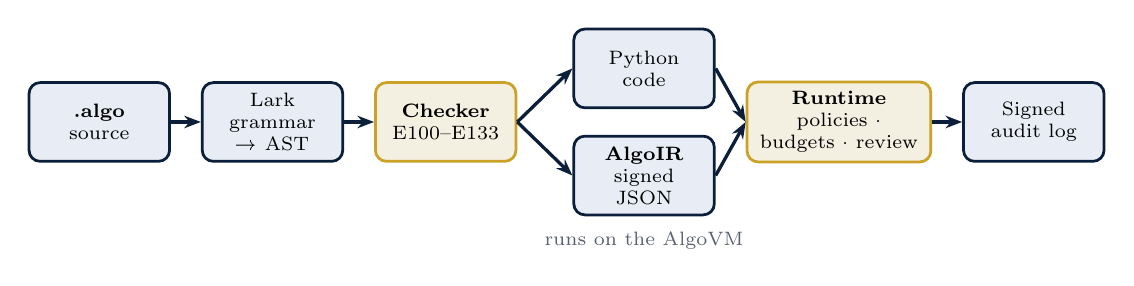
\begin{tikzpicture}[node distance=0.38cm,
  b/.style={draw=navy,line width=1pt,rounded corners=4pt,fill=navylight,minimum height=1.0cm,text width=1.55cm,align=center,font=\scriptsize},
  g/.style={b,fill=goldlight,draw=gold},a/.style={-{Stealth[length=6pt]},navy,line width=1.2pt}]
\node[b] (s) {\textbf{.algo}\\source};
\node[b,right=of s] (p) {Lark\\grammar → AST};
\node[g,right=of p] (c) {\textbf{Checker}\\E100–E133};
\node[b,right=0.7cm of c,yshift=0.68cm] (py) {Python\\code};
\node[b,right=0.7cm of c,yshift=-0.68cm] (ir) {\textbf{AlgoIR}\\signed JSON};
\node[g,right=2.9cm of c,text width=2.1cm] (rt) {\textbf{Runtime}\\policies · budgets · review};
\node[b,right=of rt] (au) {Signed\\audit log};
\draw[a] (s)--(p); \draw[a] (p)--(c); \draw[a] (c.east)--(py.west); \draw[a] (c.east)--(ir.west);
\draw[a] (py.east)--(rt.west); \draw[a] (ir.east)--(rt.west); \node[font=\scriptsize,text=muted,below=2pt of ir] {runs on the AlgoVM}; \draw[a] (rt)--(au);
\end{tikzpicture}

\vspace{10pt}
\begin{columns}[T]
\column{0.32\textwidth}\goldbox{3.9cm}{\small\textbf{34 compile-time checks}: undeclared tools, budgets, forbidden attributes, type errors, unsafe high-risk programs.}
\column{0.32\textwidth}\goldbox{3.9cm}{\small\textbf{Two engines, same result}: compiled Python or the AlgoVM; 222 programs identical in CI.}
\column{0.32\textwidth}\goldbox{3.9cm}{\small\textbf{Backends}: Claude, OpenAI-compatible local models, offline mock, replay from traces.}
\end{columns}
\end{frame}

% ═════════════════════════════ 8 · Governance ═════════════════════════════
\begin{frame}{Governance built into the language}
\footnotesize
\begin{tabularx}{\textwidth}{>{\leavevmode\color{navy}\bfseries}L{3.2cm}Y>{\raggedright\arraybackslash\ttfamily\color{navy2}}p{4.1cm}}
\toprule
\rowcolor{navy}\color{white}Control & \leavevmode\color{white}\bfseries What it does & \leavevmode\color{white}\bfseries Syntax\\
Token, cost, energy budgets & checked before every call; INR and USD; Wh and CO\textsubscript{2} & budget cost 0.04 usd\\
\rowcolor{goldlight}Forbidden attributes & a protected attribute in a goal or prompt does not compile & forbid gender, caste\\
Human review & by rule, by confidence, or always; a persistent review queue & require human when confidence < 0.8\\
\rowcolor{goldlight}Four-eyes approval & two different people must approve & require approvals 2\\
Tool permissions & only declared tools; untrusted tools are fenced & tool web.fetch untrusted\\
\rowcolor{goldlight}Organisation policy & org-wide caps that no program can loosen & algo.config.json\\
Risk levels & minimal · limited · high, each with required safeguards & risk high "purpose"\\
\bottomrule
\end{tabularx}
\end{frame}

% ═════════════════════════════ 9 · Trustworthy ═════════════════════════════
\begin{frame}{Trustworthy AI (v0.4)}{Trustworthiness as evidence, not a claim}
\begin{columns}[T]
\column{0.5\textwidth}
\begin{itemize}\setlength\itemsep{5pt}
\item \textbf{Risk levels} that change what the compiler demands.
\item \textbf{Privacy}: \texttt{redact pii}; protected values withheld even with typos.
\item \textbf{Explanations}: \texttt{explain with evidence} quotes inputs and tool results.
\item \textbf{Untrusted tools} fenced against prompt injection; MCP servers pinned by SHA-256.
\end{itemize}
\column{0.5\textwidth}
\begin{itemize}\setlength\itemsep{5pt}
\item \textbf{Signed audit}: Ed25519, and since v0.6 ML-DSA (FIPS 204) or hybrid post-quantum signatures.
\item \textbf{Retention}: audit and trace retention with signed checkpoints.
\item \textbf{System cards} and \textbf{trust reports} generated from the program itself.
\item \textbf{Evidence packs}: signed zip for auditors, verifiable offline.
\end{itemize}
\end{columns}
\end{frame}

% ═════════════════════════════ 10 · Evals ═════════════════════════════
\begin{frame}[fragile]{Uncertainty and evals}{Quality, fairness and robustness tested like code}
\begin{columns}[T]
\column{0.52\textwidth}
\begin{lstlisting}[language=AlgoLang]
eval trust on main {
    case "salaried" (app = "APP-3101 ...") {
        expect status ok
        expect fair across gender [woman, man]
        expect robust (typos, paraphrase, reorder)
               consistency >= 0.9
        expect explained
    }
}
\end{lstlisting}
\column{0.45\textwidth}
\begin{tikzpicture}
\node[fill=termbg,rounded corners=4pt,inner sep=7pt,text width=6.3cm,font=\ttfamily\scriptsize,text=termfg,align=left]{
\textcolor{gold}{\$} algo eval programs/loan\_decision.algo\\
\textcolor{green!70!white}{✓} salaried applicant\\
\quad fair across gender: same decision, gap 0.000\\
\quad robust to typos, paraphrase, reorder:\\
\quad consistency 1.00 over 6 variants\\
\textcolor{green!70!white}{✓} self-employed applicant\\
\textcolor{gold}{\quad 2/2 cases pass}};
\end{tikzpicture}
\vspace{4pt}

\small \texttt{uncertain<T>} samples an agent several times; flows branch on \texttt{.confidence}; low confidence goes to a person.
\end{columns}
\end{frame}

% ═════════════════════════════ 11 · v1.0 types ═════════════════════════════
\begin{frame}[fragile]{Typed agent-to-agent messages (v1.0)}
\begin{columns}[T]
\column{0.58\textwidth}
\begin{lstlisting}[language=AlgoLang]
type Party { name: text, phone_verified: bool }
type Claim { policy: text, amount: number,
             fraud_risk: score, claimant: Party }

agent Intake(note: text) -> Claim {
    goal "Fill in every field of the claim in {note}"
}
flow main(note: text) {
    claim = Intake(note)
    if claim.amount < 50000 and claim.fraud_risk < 0.7 {
        emit FastTrack(claim)
    } else {
        emit Investigate(claim, claim.amount)
    }
}
\end{lstlisting}
\column{0.39\textwidth}
\begin{itemize}\setlength\itemsep{5pt}\small
\item Fields and argument types checked by the compiler (E131, E132).
\item Every model answer validated against the type at run time.
\item The live model is told the exact JSON shape.
\item PII masked field by field.
\end{itemize}
\end{columns}
\end{frame}

% ═════════════════════════════ 12 · Releases features ═════════════════════════════
\begin{frame}{Beyond the core}{Real-time events, Quantum AI, interoperability and the ecosystem}
\begin{columns}[T]
\column{0.24\textwidth}\goldbox{2.85cm}{\textbf{\color{navy}AlgoPulse™}\\[2pt]\scriptsize Event streams in the language: topics, keys, dedupe, escalation and dead-letter topics, back-pressure.}
\column{0.24\textwidth}\goldbox{2.85cm}{\textbf{\color{navy}Quantum AI}\\[2pt]\scriptsize Simulator, noisy simulators, IBM, Braket and Azure backends; QPU budgets; VERIFIED / BOUNDED answers; VQE, kernels, QAOA.}
\column{0.24\textwidth}\goldbox{2.85cm}{\textbf{\color{navy}Interoperability}\\[2pt]\scriptsize Flows and agents as MCP servers; typed inputs; token streaming; cost and energy dashboard.}
\column{0.24\textwidth}\goldbox{2.85cm}{\textbf{\color{navy}Ecosystem}\\[2pt]\scriptsize AlgoIR + AlgoVM, signed packages and registry, Studio with SSO and roles, VS Code, Python SDK.}
\end{columns}
\vspace{8pt}
{\scriptsize\color{muted}Quantum hardware backends are exercised in CI with stand-in SDKs; they need the provider's credentials to run on a real device. No quantum speed-up is claimed: quantum answers are checked before use.}
\end{frame}

% ═════════════════════════════ 13 · Comparison: general languages ═════════════════════════════
\begin{frame}{Comparison with general-purpose languages}{What each language is designed for}
\scriptsize\renewcommand{\arraystretch}{1.25}
\begin{tabularx}{\textwidth}{>{\leavevmode\color{navy}\bfseries}L{1.9cm}L{2.6cm}L{2.5cm}L{2.6cm}Y}
\toprule
\rowcolor{navy}\color{white}Language & \leavevmode\color{white}\bfseries Paradigm & \leavevmode\color{white}\bfseries Typing & \leavevmode\color{white}\bfseries Concurrency & \leavevmode\color{white}\bfseries Strength \\
\rowcolor{goldlight}AlgoLang & agent-oriented, declarative flows & static: text, score, list, json, number, typed messages & \texttt{par}, \texttt{par for}, streams & governed AI decisions: policies, review, audit, evals\\
Python & multi-paradigm & dynamic (optional hints) & threads, asyncio, processes & ecosystem for AI, data and scripting\\
\rowcolor{goldlight}Java & object-oriented & static & threads, virtual threads & large enterprise systems on the JVM\\
C / C++ & procedural / multi-paradigm & static & threads & performance, systems, embedded\\
\rowcolor{goldlight}JavaScript / TS & multi-paradigm & dynamic / static (TS) & event loop, async/await & web and full-stack applications\\
Rust & multi-paradigm, ownership & static & threads, async; data-race freedom & memory safety without a garbage collector\\
\rowcolor{goldlight}Go & procedural, CSP & static & goroutines and channels & cloud services and tooling\\
\bottomrule
\end{tabularx}
\vspace{4pt}

{\scriptsize\color{muted}AlgoLang is a domain-specific language: it orchestrates AI agents and delegates computation to tools written in general-purpose languages.}
\end{frame}

% ═════════════════════════════ 14 · Comparison: scientific / AI ═════════════════════════════
\begin{frame}{Comparison with scientific, logic and AI-specific languages}
\scriptsize\renewcommand{\arraystretch}{1.2}
\begin{tabularx}{\textwidth}{>{\leavevmode\color{navy}\bfseries}L{1.8cm}L{2.8cm}Y L{4.2cm}}
\toprule
\rowcolor{navy}\color{white}Language & \leavevmode\color{white}\bfseries Focus & \leavevmode\color{white}\bfseries Core idea & \leavevmode\color{white}\bfseries Relation to AlgoLang\\
\rowcolor{goldlight}AlgoLang & governed AI agents & agents with policies; uncertainty and evals as language features & ---\\
R & statistics & vectorised data analysis, rich statistical libraries & tools for analysis inside agents\\
\rowcolor{goldlight}Julia & scientific computing & multiple dispatch, JIT compilation & numerical tools inside agents\\
MATLAB & engineering maths & matrices, toolboxes & engineering tools inside agents\\
\rowcolor{goldlight}SQL & data querying & declarative relational queries & data access tools for agents\\
Prolog & logic programming & facts, rules, unification & symbolic rules beside model agents\\
\rowcolor{goldlight}Lisp & symbolic AI & code as data, macros & historic AI language; no governance layer\\
LMQL & constrained LLM prompting & queries with constraints on model output & prompt-level; AlgoLang is program-level\\
\rowcolor{goldlight}Q\# / Qiskit & quantum programming & quantum circuits and algorithms & AlgoLang calls circuits as verified tools\\
\bottomrule
\end{tabularx}
\end{frame}

% ═════════════════════════════ 15 · Agent frameworks ═════════════════════════════
\begin{frame}{Comparison with agent frameworks}{Libraries on a host language vs.\ a language with guarantees}
\footnotesize\renewcommand{\arraystretch}{1.04}
\begin{tabularx}{\textwidth}{>{\leavevmode\color{navy}\bfseries}L{2.6cm}L{2.6cm}Y L{3.8cm}}
\toprule
\rowcolor{navy}\color{white}Framework & \leavevmode\color{white}\bfseries Form & \leavevmode\color{white}\bfseries Approach & \leavevmode\color{white}\bfseries Governance\\
\rowcolor{goldlight}AlgoLang & language + compiler & agents and flows as syntax; checked before running & built in: compile-time and run-time\\
LangChain / LangGraph & Python, JS library & chains and stateful agent graphs & added by the developer in code\\
\rowcolor{goldlight}CrewAI & Python library & role-based crews of agents & added by the developer in code\\
AutoGen & Python, .NET library & multi-agent conversations & added by the developer in code\\
\rowcolor{goldlight}Semantic Kernel & C\#, Python, Java SDK & plugins and planners in enterprise apps & added by the developer in code\\
DSPy & Python library & declarative LM programs, optimised prompts & added by the developer in code\\
\bottomrule
\end{tabularx}
\vspace{6pt}

\goldbox{13.6cm}{\small Frameworks are powerful and mature, and have far larger communities. AlgoLang's difference is \textbf{where} the guarantees live: in a compiler that refuses an unsafe program, instead of in conventions each team must remember to follow.}
\end{frame}

% ═════════════════════════════ 16 · Matrix ═════════════════════════════
\begin{frame}{Feature matrix}{\yes\ built in \quad \partly\ via libraries or conventions \quad \no\ not available}
\scriptsize\renewcommand{\arraystretch}{1.22}
\setlength\tabcolsep{4pt}
\begin{tabularx}{\textwidth}{>{\leavevmode\color{navy}\bfseries}X*{8}{>{\centering\arraybackslash}p{1.0cm}}}
\toprule
\rowcolor{navy}\color{white}Capability & \leavevmode\color{white}\bfseries AlgoLang & \leavevmode\color{white}\bfseries Python & \leavevmode\color{white}\bfseries Java & \leavevmode\color{white}\bfseries Rust & \leavevmode\color{white}\bfseries TS & \leavevmode\color{white}\bfseries Julia & \leavevmode\color{white}\bfseries Lang\-Graph & \leavevmode\color{white}\bfseries CrewAI\\
Agents as a language construct & \yes & \no & \no & \no & \no & \no & \partly & \partly\\
\rowcolor{goldlight}Budgets checked before running & \yes & \no & \no & \no & \no & \no & \partly & \partly\\
Human review / four-eyes & \yes & \partly & \partly & \partly & \partly & \partly & \partly & \partly\\
\rowcolor{goldlight}Uncertainty as a type & \yes & \partly & \partly & \partly & \partly & \partly & \no & \no\\
Fairness and robustness evals & \yes & \partly & \partly & \no & \partly & \partly & \partly & \partly\\
\rowcolor{goldlight}Signed, hash-chained audit & \yes & \partly & \partly & \partly & \partly & \partly & \partly & \partly\\
Typed agent messages & \yes & \partly & \partly & \partly & \partly & \partly & \partly & \partly\\
\rowcolor{goldlight}Quantum tools, verified & \yes & \partly & \partly & \partly & \partly & \partly & \no & \no\\
General-purpose computing & \no & \yes & \yes & \yes & \yes & \yes & \partly & \partly\\
\rowcolor{goldlight}Mature ecosystem and community & \no & \yes & \yes & \yes & \yes & \yes & \yes & \yes\\
Raw performance & \partly & \partly & \yes & \yes & \partly & \yes & \partly & \partly\\
\bottomrule
\end{tabularx}
\end{frame}

% ═════════════════════════════ 17 · Side by side ═════════════════════════════
\begin{frame}[fragile]{The same guarantee, two ways}{A budgeted agent with human review on low confidence}
\begin{columns}[T]
\column{0.5\textwidth}
\textbf{\color{navy}Python with a framework} {\scriptsize\color{muted}(sketch)}
\begin{lstlisting}[style=py]
def triage(claim):
    if tokens_used() > 2000:
        raise BudgetError()
    out = llm.invoke(prompt(claim))
    score, conf = parse(out)
    log_audit(claim, out)        # remember to sign
    if conf < 0.8:
        queue_for_review(out)    # remember to persist
    if "gender" in prompt(claim):
        ...                      # remember to check
    return score
\end{lstlisting}
\column{0.47\textwidth}
\textbf{\color{navy}AlgoLang}
\begin{lstlisting}[language=AlgoLang]
agent Triage(claim: text) -> uncertain<score> {
    goal   "Score {claim}"
    policy { budget tokens 2000
             require human when confidence < 0.8
             forbid gender }
}
\end{lstlisting}
\vspace{4pt}
\small Budget, review queue, forbidden attribute and signed audit are \textbf{enforced}, not remembered.
\end{columns}
\end{frame}

% ═════════════════════════════ 18 · Not the right tool ═════════════════════════════
\begin{frame}{Where AlgoLang is not the right tool}{An honest view}
\begin{columns}[T]
\column{0.5\textwidth}
\begin{itemize}\setlength\itemsep{6pt}
\item \textbf{General computation.} No loops over numbers, no data structures beyond its types: write those as tools in Python or another language.
\item \textbf{High-performance code.} The runtime is Python; speed comes from tools.
\item \textbf{A young ecosystem.} One maintainer team, a small community and few third-party packages so far.
\end{itemize}
\column{0.5\textwidth}
\goldbox{6.1cm}{\textbf{\color{navy}Use AlgoLang when}\\[3pt]\small
\textcolor{gold}{■} AI agents make decisions that affect people or money\\
\textcolor{gold}{■} you must show regulators who decided and why\\
\textcolor{gold}{■} fairness, budgets and human review are requirements, not wishes\\
\textcolor{gold}{■} you want agent programs that are reviewed and tested like code}
\end{columns}
\end{frame}

% ═════════════════════════════ 19 · Applications ═════════════════════════════
\begin{frame}{22 governed enterprise applications}{Each with policies, company tools, knowledge base, evals, behaviour tests and system cards}
\scriptsize
\begin{columns}[T]
\column{0.33\textwidth}
\textbf{\color{navy}Enterprise}
\begin{itemize}\setlength\itemsep{1pt}
\item Insurance claims operations
\item Hospital care coordination
\item Bank credit and KYC
\item University admissions and OBE
\item SOC incident command
\item Supply chain control tower
\item Citizen services
\item Legal contract desk
\end{itemize}
\column{0.33\textwidth}
\textbf{\color{navy}AI, markets and quantum}
\begin{itemize}\setlength\itemsep{1pt}
\item Algo trading desk
\item Quantum optimization lab
\item AlgoQ Quantum AI lab
\item AlgoGraph LLM \& SLM optimizer
\item ML model factory
\item RL control room
\item Responsible XAI studio
\item NLP document intelligence
\end{itemize}
\column{0.33\textwidth}
\textbf{\color{navy}Large-scale domains (v0.5)}
\begin{itemize}\setlength\itemsep{1pt}
\item Bharat language desk (8 scripts)
\item Digital health monitor (NEWS2)
\item Network biology lab
\item Predictive maintenance
\item Smart city operations
\item Transport network optimizer
\end{itemize}
\end{columns}
\vspace{6pt}
\begin{center}\stat{22}{applications}\quad\stat{38}{programs}\quad\stat{222}{programs on AlgoVM}\quad\stat{34}{compile checks}\end{center}
\end{frame}

% Generated by make_apps_tex.py from apps.json: do not edit by hand.

\begin{frame}{Applications · Enterprise operations}{enterprise-apps/claims-ops-center, hospital-care-coordination}
\begin{columns}[T,onlytextwidth]
\column{0.49\textwidth}
\begin{tcolorbox}[appcard,equal height group=apps1]
{\fontsize{6.5}{8}\selectfont\color{muted}01\,/\,22}\hfill\riskpill{gold!85!black}{LIMITED RISK}\\[1pt]
{\normalsize\bfseries\color{navy}Claims Operations Center}\\[-1pt]
{\scriptsize\bfseries\color{gold!85!black}Insurance}\par\vspace{3pt}
{\scriptsize\textbf{\color{navy}Challenge}\enspace First notice of loss takes hours: policy checks, fraud screening and a fair payout estimate.\par}\vspace{2pt}
{\fontsize{6.5}{8}\selectfont\bfseries\color{muted}WHAT IT DOES}
\begin{itemize}\setlength\itemsep{0pt}\scriptsize
\item Reads the claim and pulls cover, deductible and status from the policy database
\item A three-member fraud panel runs in parallel
\item High fraud score $\rightarrow$ SIU referral note, and the flow stops
\end{itemize}
\vspace{1pt}\govbox{Payout drafts carry evidence; fraud referrals stop automation}\par\vspace{3pt}
{\fontsize{6.5}{8}\selectfont\ttfamily\color{navy2}policydb.lookup\enspace payout.estimate}\hfill{\fontsize{6.5}{8}\selectfont\color{muted}2 programs}
\end{tcolorbox}
\column{0.49\textwidth}
\begin{tcolorbox}[appcard,equal height group=apps1]
{\fontsize{6.5}{8}\selectfont\color{muted}02\,/\,22}\hfill\riskpill{badred}{HIGH RISK}\\[1pt]
{\normalsize\bfseries\color{navy}Hospital Care Coordination}\\[-1pt]
{\scriptsize\bfseries\color{gold!85!black}Healthcare}\par\vspace{3pt}
{\scriptsize\textbf{\color{navy}Challenge}\enspace Emergency departments must triage fast, find a bed, hand over cleanly and write discharge summaries.\par}\vspace{2pt}
{\fontsize{6.5}{8}\selectfont\bfseries\color{muted}WHAT IT DOES}
\begin{itemize}\setlength\itemsep{0pt}\scriptsize
\item Extracts key facts from the ER note into a structured summary
\item Scores urgency; urgent cases get a live bed and a referral draft
\item Drafts discharge summaries for clinician sign-off
\end{itemize}
\vspace{1pt}\govbox{Every score below threshold goes to the duty clinician}\par\vspace{3pt}
{\fontsize{6.5}{8}\selectfont\ttfamily\color{navy2}file.read\enspace beds.availability}\hfill{\fontsize{6.5}{8}\selectfont\color{muted}2 programs}
\end{tcolorbox}
\end{columns}
\end{frame}

\begin{frame}{Applications · Enterprise operations}{enterprise-apps/bank-credit-onboarding, university-admissions-obe}
\begin{columns}[T,onlytextwidth]
\column{0.49\textwidth}
\begin{tcolorbox}[appcard,equal height group=apps2]
{\fontsize{6.5}{8}\selectfont\color{muted}03\,/\,22}\hfill\riskpill{badred}{HIGH RISK}\\[1pt]
{\normalsize\bfseries\color{navy}Bank Credit \& Onboarding}\\[-1pt]
{\scriptsize\bfseries\color{gold!85!black}Banking}\par\vspace{3pt}
{\scriptsize\textbf{\color{navy}Challenge}\enspace Loan and KYC decisions need bureau data, affordability maths and sanctions screening, all explainable.\par}\vspace{2pt}
{\fontsize{6.5}{8}\selectfont\bfseries\color{muted}WHAT IT DOES}
\begin{itemize}\setlength\itemsep{0pt}\scriptsize
\item Pulls the bureau record and computes EMI and debt-to-income
\item Credit, risk and policy analysts review in parallel
\item Credit committee scores the case and writes a decision memo
\end{itemize}
\vspace{1pt}\govbox{Gender and religion forbidden; low confidence $\rightarrow$ a person}\par\vspace{3pt}
{\fontsize{6.5}{8}\selectfont\ttfamily\color{navy2}bureau.score\enspace dti.calc\enspace sanctions.screen}\hfill{\fontsize{6.5}{8}\selectfont\color{muted}2 programs}
\end{tcolorbox}
\column{0.49\textwidth}
\begin{tcolorbox}[appcard,equal height group=apps2]
{\fontsize{6.5}{8}\selectfont\color{muted}04\,/\,22}\hfill\riskpill{badred}{HIGH RISK}\\[1pt]
{\normalsize\bfseries\color{navy}University Admissions \& OBE}\\[-1pt]
{\scriptsize\bfseries\color{gold!85!black}Higher education}\par\vspace{3pt}
{\scriptsize\textbf{\color{navy}Challenge}\enspace Admissions must be merit-based and fair, and every course needs NBA/NAAC outcome-based evidence.\par}\vspace{2pt}
{\fontsize{6.5}{8}\selectfont\bfseries\color{muted}WHAT IT DOES}
\begin{itemize}\setlength\itemsep{0pt}\scriptsize
\item Checks seats and merit cut-offs for the programme
\item Academic, statement and potential reviewers assess in parallel
\item Panel scores the case and drafts the letter; CO-PO attainment for OBE
\end{itemize}
\vspace{1pt}\govbox{Caste, gender, religion, nationality, income: forbidden inputs}\par\vspace{3pt}
{\fontsize{6.5}{8}\selectfont\ttfamily\color{navy2}seats.lookup\enspace file.read}\hfill{\fontsize{6.5}{8}\selectfont\color{muted}2 programs}
\end{tcolorbox}
\end{columns}
\end{frame}

\begin{frame}{Applications · Enterprise operations}{enterprise-apps/soc-incident-command, supply-chain-control-tower}
\begin{columns}[T,onlytextwidth]
\column{0.49\textwidth}
\begin{tcolorbox}[appcard,equal height group=apps3]
{\fontsize{6.5}{8}\selectfont\color{muted}05\,/\,22}\hfill\riskpill{gold!85!black}{LIMITED RISK}\\[1pt]
{\normalsize\bfseries\color{navy}SOC Incident Command}\\[-1pt]
{\scriptsize\bfseries\color{gold!85!black}Cybersecurity \& IT operations}\par\vspace{3pt}
{\scriptsize\textbf{\color{navy}Challenge}\enspace Security operations centres drown in alerts; analysts need assets, owners and threat intel at once.\par}\vspace{2pt}
{\fontsize{6.5}{8}\selectfont\bfseries\color{muted}WHAT IT DOES}
\begin{itemize}\setlength\itemsep{0pt}\scriptsize
\item Enriches alerts from the CMDB and checks every IP and domain against threat intel
\item Splits the batch and scores severity in parallel
\item Severe $\rightarrow$ IT operations runbook; post-quantum readiness scan
\end{itemize}
\vspace{1pt}\govbox{Untrusted intel fenced against prompt injection}\par\vspace{3pt}
{\fontsize{6.5}{8}\selectfont\ttfamily\color{navy2}cmdb.lookup\enspace ioc.check\enspace pqc.scan}\hfill{\fontsize{6.5}{8}\selectfont\color{muted}3 programs}
\end{tcolorbox}
\column{0.49\textwidth}
\begin{tcolorbox}[appcard,equal height group=apps3]
{\fontsize{6.5}{8}\selectfont\color{muted}06\,/\,22}\hfill\riskpill{okgreen}{MINIMAL RISK}\\[1pt]
{\normalsize\bfseries\color{navy}Supply Chain Control Tower}\\[-1pt]
{\scriptsize\bfseries\color{gold!85!black}Logistics \& retail}\par\vspace{3pt}
{\scriptsize\textbf{\color{navy}Challenge}\enspace Customs holds, breakdowns and damage need a quick view of where stock is and what to do next.\par}\vspace{2pt}
{\fontsize{6.5}{8}\selectfont\bfseries\color{muted}WHAT IT DOES}
\begin{itemize}\setlength\itemsep{0pt}\scriptsize
\item Tracks the shipment and checks stock cover in parallel
\item Scores how critical the exception is
\item Critical $\rightarrow$ impact, alternatives, costs and a recovery plan
\end{itemize}
\vspace{1pt}\govbox{Quantum route options verified before they are proposed}\par\vspace{3pt}
{\fontsize{6.5}{8}\selectfont\ttfamily\color{navy2}shipment.track\enspace inventory.levels\enspace quantum.routes}\hfill{\fontsize{6.5}{8}\selectfont\color{muted}2 programs}
\end{tcolorbox}
\end{columns}
\end{frame}

\begin{frame}{Applications · Enterprise operations}{enterprise-apps/citizen-services-desk, legal-contract-desk}
\begin{columns}[T,onlytextwidth]
\column{0.49\textwidth}
\begin{tcolorbox}[appcard,equal height group=apps4]
{\fontsize{6.5}{8}\selectfont\color{muted}07\,/\,22}\hfill\riskpill{badred}{HIGH RISK}\\[1pt]
{\normalsize\bfseries\color{navy}Citizen Services Desk}\\[-1pt]
{\scriptsize\bfseries\color{gold!85!black}Government \& public services}\par\vspace{3pt}
{\scriptsize\textbf{\color{navy}Challenge}\enspace Complaints must reach the right department fast; urgent ones (health, safety, children) first.\par}\vspace{2pt}
{\fontsize{6.5}{8}\selectfont\bfseries\color{muted}WHAT IT DOES}
\begin{itemize}\setlength\itemsep{0pt}\scriptsize
\item Finds ward, department, desk and service-level target
\item Urgent $\rightarrow$ priority cell with an action plan
\item Checks every reply for clarity; welfare eligibility pre-check
\end{itemize}
\vspace{1pt}\govbox{AI disclosure on every reply; eligibility decided by people}\par\vspace{3pt}
{\fontsize{6.5}{8}\selectfont\ttfamily\color{navy2}ward.directory}\hfill{\fontsize{6.5}{8}\selectfont\color{muted}2 programs}
\end{tcolorbox}
\column{0.49\textwidth}
\begin{tcolorbox}[appcard,equal height group=apps4]
{\fontsize{6.5}{8}\selectfont\color{muted}08\,/\,22}\hfill\riskpill{okgreen}{MINIMAL RISK}\\[1pt]
{\normalsize\bfseries\color{navy}Legal Contract Desk}\\[-1pt]
{\scriptsize\bfseries\color{gold!85!black}Legal \& compliance}\par\vspace{3pt}
{\scriptsize\textbf{\color{navy}Challenge}\enspace In-house legal teams review dozens of NDAs and contracts a week against the same playbook.\par}\vspace{2pt}
{\fontsize{6.5}{8}\selectfont\bfseries\color{muted}WHAT IT DOES}
\begin{itemize}\setlength\itemsep{0pt}\scriptsize
\item Extracts NDA terms and scores deviation from the playbook
\item Suggests redlines with approved fallback wording
\item Analyses every contract clause in parallel and summarises for counsel
\end{itemize}
\vspace{1pt}\govbox{Counsel decides; the desk drafts with cited clauses}\par\vspace{3pt}
{\fontsize{6.5}{8}\selectfont\ttfamily\color{navy2}clause.library\enspace file.read}\hfill{\fontsize{6.5}{8}\selectfont\color{muted}2 programs}
\end{tcolorbox}
\end{columns}
\end{frame}

\begin{frame}{Applications · AI, markets \& quantum}{enterprise-apps/algo-trading-desk, quantum-optimization-lab}
\begin{columns}[T,onlytextwidth]
\column{0.49\textwidth}
\begin{tcolorbox}[appcard,equal height group=apps5]
{\fontsize{6.5}{8}\selectfont\color{muted}09\,/\,22}\hfill\riskpill{okgreen}{MINIMAL RISK}\\[1pt]
{\normalsize\bfseries\color{navy}Algo Trading Desk (QuantOracle™)}\\[-1pt]
{\scriptsize\bfseries\color{gold!85!black}Capital markets}\par\vspace{3pt}
{\scriptsize\textbf{\color{navy}Challenge}\enspace A trading desk must decide which strategies are robust enough to trade, within risk and conduct rules.\par}\vspace{2pt}
{\fontsize{6.5}{8}\selectfont\bfseries\color{muted}WHAT IT DOES}
\begin{itemize}\setlength\itemsep{0pt}\scriptsize
\item Quant, compliance and editorial reviewers run in parallel
\item Robustness is an \texttt{uncertain<score>} sampled five times
\item Failing backtests (PF < 1.3 or DD > 15\%) are rejected by a guard
\end{itemize}
\vspace{1pt}\govbox{Approval only for PAPER trading, through the review queue}\par\vspace{3pt}
{\fontsize{6.5}{8}\selectfont\ttfamily\color{navy2}backtest.stats\enspace risk.limits\enspace market.quote}\hfill{\fontsize{6.5}{8}\selectfont\color{muted}4 programs}
\end{tcolorbox}
\column{0.49\textwidth}
\begin{tcolorbox}[appcard,equal height group=apps5]
{\fontsize{6.5}{8}\selectfont\color{muted}10\,/\,22}\hfill\riskpill{okgreen}{MINIMAL RISK}\\[1pt]
{\normalsize\bfseries\color{navy}Quantum Optimization Lab}\\[-1pt]
{\scriptsize\bfseries\color{gold!85!black}Quantum for finance \& operations}\par\vspace{3pt}
{\scriptsize\textbf{\color{navy}Challenge}\enspace Many business decisions are combinatorial: which k of n assets to hold, which jobs go on which shift.\par}\vspace{2pt}
{\fontsize{6.5}{8}\selectfont\bfseries\color{muted}WHAT IT DOES}
\begin{itemize}\setlength\itemsep{0pt}\scriptsize
\item Portfolio selection as a QUBO, solved with QAOA
\item Max-cut, scheduling and certified quantum randomness
\item Every answer checked against the exact classical optimum
\end{itemize}
\vspace{1pt}\govbox{Guard on VERIFIED / GAP; max qubits enforced by policy}\par\vspace{3pt}
{\fontsize{6.5}{8}\selectfont\ttfamily\color{navy2}quantum.portfolio\enspace quantum.qubo\enspace quantum.maxcut}\hfill{\fontsize{6.5}{8}\selectfont\color{muted}4 programs}
\end{tcolorbox}
\end{columns}
\end{frame}

\begin{frame}{Applications · AI, markets \& quantum}{enterprise-apps/quantum-ai-lab, llm-graph-optimizer}
\begin{columns}[T,onlytextwidth]
\column{0.49\textwidth}
\begin{tcolorbox}[appcard,equal height group=apps6]
{\fontsize{6.5}{8}\selectfont\color{muted}11\,/\,22}\hfill\riskpill{okgreen}{MINIMAL RISK}\\[1pt]
{\normalsize\bfseries\color{navy}AlgoQ Quantum AI Lab™}\\[-1pt]
{\scriptsize\bfseries\color{gold!85!black}Quantum computing}\par\vspace{3pt}
{\scriptsize\textbf{\color{navy}Challenge}\enspace Quantum computers are noisy, scarce and expensive, and their answers are distributions, not facts.\par}\vspace{2pt}
{\fontsize{6.5}{8}\selectfont\bfseries\color{muted}WHAT IT DOES}
\begin{itemize}\setlength\itemsep{0pt}\scriptsize
\item VQE ground-state energies, checked by exact diagonalisation
\item Knapsack capital budgeting and spectrum colouring with QAOA
\item Quantum kernels cross-validated against a classical RBF
\end{itemize}
\vspace{1pt}\govbox{QPU budgets; only VERIFIED answers reach a two-approval committee}\par\vspace{3pt}
{\fontsize{6.5}{8}\selectfont\ttfamily\color{navy2}quantum.vqe\enspace quantum.kernel\enspace quantum.knapsack}\hfill{\fontsize{6.5}{8}\selectfont\color{muted}1 program}
\end{tcolorbox}
\column{0.49\textwidth}
\begin{tcolorbox}[appcard,equal height group=apps6]
{\fontsize{6.5}{8}\selectfont\color{muted}12\,/\,22}\hfill\riskpill{gold!85!black}{LIMITED RISK}\\[1pt]
{\normalsize\bfseries\color{navy}AlgoGraph™ LLM \& SLM Optimizer}\\[-1pt]
{\scriptsize\bfseries\color{gold!85!black}AI platform engineering · MLOps}\par\vspace{3pt}
{\scriptsize\textbf{\color{navy}Challenge}\enspace Large models are slow and costly; small models are cheap but not always good enough.\par}\vspace{2pt}
{\fontsize{6.5}{8}\selectfont\bfseries\color{muted}WHAT IT DOES}
\begin{itemize}\setlength\itemsep{0pt}\scriptsize
\item Reads each program's agent graph from the compiler
\item Picks the cheapest LLM or SLM per agent that meets quality and latency
\item Proves the choice optimal; routes live traffic small-model-first
\end{itemize}
\vspace{1pt}\govbox{Route decided in code, not by a model}\par\vspace{3pt}
{\fontsize{6.5}{8}\selectfont\ttfamily\color{navy2}graph.analyze\enspace graph.optimize\enspace slm.triage}\hfill{\fontsize{6.5}{8}\selectfont\color{muted}2 programs}
\end{tcolorbox}
\end{columns}
\end{frame}

\begin{frame}{Applications · AI, markets \& quantum}{enterprise-apps/ml-model-factory, rl-control-room}
\begin{columns}[T,onlytextwidth]
\column{0.49\textwidth}
\begin{tcolorbox}[appcard,equal height group=apps7]
{\fontsize{6.5}{8}\selectfont\color{muted}13\,/\,22}\hfill\riskpill{gold!85!black}{LIMITED RISK}\\[1pt]
{\normalsize\bfseries\color{navy}AlgoML Model Factory™}\\[-1pt]
{\scriptsize\bfseries\color{gold!85!black}Machine learning \& deep learning}\par\vspace{3pt}
{\scriptsize\textbf{\color{navy}Challenge}\enspace Shipping a model safely needs more than a high score: fair comparison, calibration and drift checks.\par}\vspace{2pt}
{\fontsize{6.5}{8}\selectfont\bfseries\color{muted}WHAT IT DOES}
\begin{itemize}\setlength\itemsep{0pt}\scriptsize
\item Trains three model families in parallel with 5-fold cross-validation
\item Picks a calibrated champion (ECE $\le$ 0.05)
\item Catches target leakage before training; monitors drift
\end{itemize}
\vspace{1pt}\govbox{A leaking column stops the run before any training}\par\vspace{3pt}
{\fontsize{6.5}{8}\selectfont\ttfamily\color{navy2}ml.train\enspace ml.compare\enspace ml.drift}\hfill{\fontsize{6.5}{8}\selectfont\color{muted}1 program}
\end{tcolorbox}
\column{0.49\textwidth}
\begin{tcolorbox}[appcard,equal height group=apps7]
{\fontsize{6.5}{8}\selectfont\color{muted}14\,/\,22}\hfill\riskpill{okgreen}{MINIMAL RISK}\\[1pt]
{\normalsize\bfseries\color{navy}AlgoRL Control Room™}\\[-1pt]
{\scriptsize\bfseries\color{gold!85!black}Reinforcement learning for energy}\par\vspace{3pt}
{\scriptsize\textbf{\color{navy}Challenge}\enspace An RL controller can beat a hand-written rule, but a grid cannot afford trial-and-error mistakes.\par}\vspace{2pt}
{\fontsize{6.5}{8}\selectfont\bfseries\color{muted}WHAT IT DOES}
\begin{itemize}\setlength\itemsep{0pt}\scriptsize
\item Q-learning for a 2 MWh campus battery over 3,000 simulated days
\item Safety shield enforces the 1.75 MW grid-import cap
\item Benchmarked against the exact optimum, then heatwave stress tests
\end{itemize}
\vspace{1pt}\govbox{Policy deploys only after it beats the rule and stays safe}\par\vspace{3pt}
{\fontsize{6.5}{8}\selectfont\ttfamily\color{navy2}rl.train\enspace rl.evaluate\enspace rl.stress}\hfill{\fontsize{6.5}{8}\selectfont\color{muted}1 program}
\end{tcolorbox}
\end{columns}
\end{frame}

\begin{frame}{Applications · AI, markets \& quantum}{enterprise-apps/responsible-xai-studio, nlp-document-intelligence}
\begin{columns}[T,onlytextwidth]
\column{0.49\textwidth}
\begin{tcolorbox}[appcard,equal height group=apps8]
{\fontsize{6.5}{8}\selectfont\color{muted}15\,/\,22}\hfill\riskpill{gold!85!black}{LIMITED RISK}\\[1pt]
{\normalsize\bfseries\color{navy}AlgoXAI Audit Studio™}\\[-1pt]
{\scriptsize\bfseries\color{gold!85!black}Responsible \& explainable AI}\par\vspace{3pt}
{\scriptsize\textbf{\color{navy}Challenge}\enspace A credit model can be accurate and still unfair, often through a feature that stands in for a protected one.\par}\vspace{2pt}
{\fontsize{6.5}{8}\selectfont\bfseries\color{muted}WHAT IT DOES}
\begin{itemize}\setlength\itemsep{0pt}\scriptsize
\item Exact Shapley values over all 2\textsuperscript{6} coalitions
\item Fairness audit on a group used only for auditing
\item Actionable recourse: the smallest change that flips a decline
\end{itemize}
\vspace{1pt}\govbox{Age and area are never suggested as changes}\par\vspace{3pt}
{\fontsize{6.5}{8}\selectfont\ttfamily\color{navy2}xai.shapley\enspace fair.audit\enspace xai.counterfactual}\hfill{\fontsize{6.5}{8}\selectfont\color{muted}1 program}
\end{tcolorbox}
\column{0.49\textwidth}
\begin{tcolorbox}[appcard,equal height group=apps8]
{\fontsize{6.5}{8}\selectfont\color{muted}16\,/\,22}\hfill\riskpill{gold!85!black}{LIMITED RISK}\\[1pt]
{\normalsize\bfseries\color{navy}AlgoNLP Document Intelligence™}\\[-1pt]
{\scriptsize\bfseries\color{gold!85!black}Natural language processing}\par\vspace{3pt}
{\scriptsize\textbf{\color{navy}Challenge}\enspace A bank receives thousands of messages a week: card blocks, loans, KYC updates, fraud reports.\par}\vspace{2pt}
{\fontsize{6.5}{8}\selectfont\bfseries\color{muted}WHAT IT DOES}
\begin{itemize}\setlength\itemsep{0pt}\scriptsize
\item Classifies, extracts entities and summarises every message in parallel
\item Emerging topics and distinctive words per category
\item Reply drafts routed to the right queue
\end{itemize}
\vspace{1pt}\govbox{Fraud reports always go to a person, with evidence}\par\vspace{3pt}
{\fontsize{6.5}{8}\selectfont\ttfamily\color{navy2}nlp.classify\enspace nlp.entities\enspace nlp.trends}\hfill{\fontsize{6.5}{8}\selectfont\color{muted}1 program}
\end{tcolorbox}
\end{columns}
\end{frame}

\begin{frame}{Applications · Large-scale domains}{enterprise-apps/bharat-language-desk, digital-health-monitor}
\begin{columns}[T,onlytextwidth]
\column{0.49\textwidth}
\begin{tcolorbox}[appcard,equal height group=apps9]
{\fontsize{6.5}{8}\selectfont\color{muted}17\,/\,22}\hfill\riskpill{gold!85!black}{LIMITED RISK}\\[1pt]
{\normalsize\bfseries\color{navy}AlgoBharat Bhasha Desk™}\\[-1pt]
{\scriptsize\bfseries\color{gold!85!black}Indian-language AI for citizen services}\par\vspace{3pt}
{\scriptsize\textbf{\color{navy}Challenge}\enspace Citizens write in their own language and script: Telugu, Hindi, Tamil, Bengali and more.\par}\vspace{2pt}
{\fontsize{6.5}{8}\selectfont\bfseries\color{muted}WHAT IT DOES}
\begin{itemize}\setlength\itemsep{0pt}\scriptsize
\item Detects the language from 11 scripts; separates Hindi from Marathi
\item Transliterates Brahmic scripts (ISO 15919 style)
\item Finds the need (pension, ration, water…) and replies in kind
\end{itemize}
\vspace{1pt}\govbox{Coverage reported honestly; unknown scripts go to a person}\par\vspace{3pt}
{\fontsize{6.5}{8}\selectfont\ttfamily\color{navy2}lang.detect\enspace lang.transliterate\enspace lang.intent}\hfill{\fontsize{6.5}{8}\selectfont\color{muted}1 program}
\end{tcolorbox}
\column{0.49\textwidth}
\begin{tcolorbox}[appcard,equal height group=apps9]
{\fontsize{6.5}{8}\selectfont\color{muted}18\,/\,22}\hfill\riskpill{badred}{HIGH RISK}\\[1pt]
{\normalsize\bfseries\color{navy}AlgoCare Remote Monitoring™}\\[-1pt]
{\scriptsize\bfseries\color{gold!85!black}Healthcare \& digital health}\par\vspace{3pt}
{\scriptsize\textbf{\color{navy}Challenge}\enspace Thousands of patients are monitored at home; their readings must be triaged safely, around the clock.\par}\vspace{2pt}
{\fontsize{6.5}{8}\selectfont\bfseries\color{muted}WHAT IT DOES}
\begin{itemize}\setlength\itemsep{0pt}\scriptsize
\item Scores every reading with NEWS2, exactly by published bands
\item Checks the record and major drug interactions in parallel
\item High $\rightarrow$ emergency alert; medium $\rightarrow$ review within the hour
\end{itemize}
\vspace{1pt}\govbox{A clinician reviews every alert}\par\vspace{3pt}
{\fontsize{6.5}{8}\selectfont\ttfamily\color{navy2}vitals.news2\enspace ehr.patient\enspace drug.check}\hfill{\fontsize{6.5}{8}\selectfont\color{muted}1 program}
\end{tcolorbox}
\end{columns}
\end{frame}

\begin{frame}{Applications · Large-scale domains}{enterprise-apps/network-biology-lab, predictive-engineering}
\begin{columns}[T,onlytextwidth]
\column{0.49\textwidth}
\begin{tcolorbox}[appcard,equal height group=apps10]
{\fontsize{6.5}{8}\selectfont\color{muted}19\,/\,22}\hfill\riskpill{okgreen}{MINIMAL RISK}\\[1pt]
{\normalsize\bfseries\color{navy}AlgoBio Network Lab™}\\[-1pt]
{\scriptsize\bfseries\color{gold!85!black}Computational \& network biology}\par\vspace{3pt}
{\scriptsize\textbf{\color{navy}Challenge}\enspace Disease genes cluster in the protein network, so known proteins can point to new candidates.\par}\vspace{2pt}
{\fontsize{6.5}{8}\selectfont\bfseries\color{muted}WHAT IT DOES}
\begin{itemize}\setlength\itemsep{0pt}\scriptsize
\item Analyses a 1,500-protein, 7,441-interaction network in parallel
\item Random walk with restart, validated on hidden disease proteins
\item Negative control from random seeds; enrichment and sequences
\end{itemize}
\vspace{1pt}\govbox{A weak control is required before results are reported}\par\vspace{3pt}
{\fontsize{6.5}{8}\selectfont\ttfamily\color{navy2}net.propagate\enspace net.modules\enspace bio.enrich}\hfill{\fontsize{6.5}{8}\selectfont\color{muted}1 program}
\end{tcolorbox}
\column{0.49\textwidth}
\begin{tcolorbox}[appcard,equal height group=apps10]
{\fontsize{6.5}{8}\selectfont\color{muted}20\,/\,22}\hfill\riskpill{okgreen}{MINIMAL RISK}\\[1pt]
{\normalsize\bfseries\color{navy}AlgoEng Predictive Maintenance™}\\[-1pt]
{\scriptsize\bfseries\color{gold!85!black}Data-driven engineering}\par\vspace{3pt}
{\scriptsize\textbf{\color{navy}Challenge}\enspace Unplanned pump failures stop production and can be dangerous; the data shows them coming.\par}\vspace{2pt}
{\fontsize{6.5}{8}\selectfont\bfseries\color{muted}WHAT IT DOES}
\begin{itemize}\setlength\itemsep{0pt}\scriptsize
\item Vibration diagnosis by ISO zones, in parallel with prognosis
\item Remaining useful life with a 90\% interval
\item Fleet scan and a maintenance plan
\end{itemize}
\vspace{1pt}\govbox{Urgent work orders are approved by a person}\par\vspace{3pt}
{\fontsize{6.5}{8}\selectfont\ttfamily\color{navy2}vib.diagnose\enspace rul.estimate\enspace maint.plan}\hfill{\fontsize{6.5}{8}\selectfont\color{muted}1 program}
\end{tcolorbox}
\end{columns}
\end{frame}

\begin{frame}{Applications · Large-scale domains}{enterprise-apps/smart-city-operations, transport-network-optimizer}
\begin{columns}[T,onlytextwidth]
\column{0.49\textwidth}
\begin{tcolorbox}[appcard,equal height group=apps11]
{\fontsize{6.5}{8}\selectfont\color{muted}21\,/\,22}\hfill\riskpill{gold!85!black}{LIMITED RISK}\\[1pt]
{\normalsize\bfseries\color{navy}AlgoCity Operations Centre™}\\[-1pt]
{\scriptsize\bfseries\color{gold!85!black}Smart cities}\par\vspace{3pt}
{\scriptsize\textbf{\color{navy}Challenge}\enspace A city control room sees air, waste and electricity data around the clock, each in its own silo.\par}\vspace{2pt}
{\fontsize{6.5}{8}\selectfont\bfseries\color{muted}WHAT IT DOES}
\begin{itemize}\setlength\itemsep{0pt}\scriptsize
\item Checks AQI (CPCB), waste routes and energy load in parallel
\item Very poor AQI $\rightarrow$ multilingual health advisory
\item Overload risk $\rightarrow$ load plan; never hospitals, water or signals
\end{itemize}
\vspace{1pt}\govbox{Advisories need the duty officer; load plans need two officers}\par\vspace{3pt}
{\fontsize{6.5}{8}\selectfont\ttfamily\color{navy2}city.aqi\enspace city.waste\enspace city.energy}\hfill{\fontsize{6.5}{8}\selectfont\color{muted}1 program}
\end{tcolorbox}
\column{0.49\textwidth}
\begin{tcolorbox}[appcard,equal height group=apps11]
{\fontsize{6.5}{8}\selectfont\color{muted}22\,/\,22}\hfill\riskpill{gold!85!black}{LIMITED RISK}\\[1pt]
{\normalsize\bfseries\color{navy}AlgoMove Transport Network Optimizer™}\\[-1pt]
{\scriptsize\bfseries\color{gold!85!black}Transportation systems}\par\vspace{3pt}
{\scriptsize\textbf{\color{navy}Challenge}\enspace When an arterial road closes, traffic floods side streets within minutes; fixed signals cannot cope.\par}\vspace{2pt}
{\fontsize{6.5}{8}\selectfont\bfseries\color{muted}WHAT IT DOES}
\begin{itemize}\setlength\itemsep{0pt}\scriptsize
\item Reroutes traffic (Dijkstra) and retimes signals (Webster) in parallel
\item Gravity-model demand and transit headways
\item Oversaturated junctions $\rightarrow$ police control and metering plan
\end{itemize}
\vspace{1pt}\govbox{Control-room officer approves; notices carry AI disclosure}\par\vspace{3pt}
{\fontsize{6.5}{8}\selectfont\ttfamily\color{navy2}traffic.reroute\enspace signal.retime\enspace demand.od}\hfill{\fontsize{6.5}{8}\selectfont\color{muted}1 program}
\end{tcolorbox}
\end{columns}
\end{frame}


% ═════════════════════════════ 20 · Toolchain ═════════════════════════════
\begin{frame}{Toolchain}
\begin{columns}[T]
\column{0.5\textwidth}
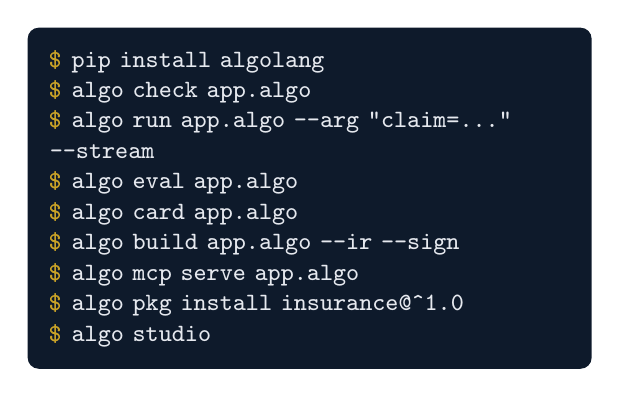
\begin{tikzpicture}
\node[fill=termbg,rounded corners=4pt,inner sep=8pt,text width=6.6cm,font=\ttfamily\small,text=termfg,align=left]{
\textcolor{gold}{\$} pip install algolang\\
\textcolor{gold}{\$} algo check app.algo\\
\textcolor{gold}{\$} algo run app.algo --arg "claim=..." --stream\\
\textcolor{gold}{\$} algo eval app.algo\\
\textcolor{gold}{\$} algo card app.algo\\
\textcolor{gold}{\$} algo build app.algo --ir --sign\\
\textcolor{gold}{\$} algo mcp serve app.algo\\
\textcolor{gold}{\$} algo pkg install insurance@\^{}1.0\\
\textcolor{gold}{\$} algo studio};
\end{tikzpicture}
\column{0.47\textwidth}
\begin{itemize}\setlength\itemsep{4pt}\small
\item \textbf{CLI} \texttt{algo}: check, run, batch, eval, card, report, audit, evidence, build, pkg, mcp.
\item \textbf{Studio}: browser IDE with review queue, dashboard, SSO and roles.
\item \textbf{Python SDK} and Jupyter / Colab.
\item \textbf{VS Code} extension and language server.
\item \textbf{CI}: Linux, macOS and Windows on every change.
\end{itemize}
\end{columns}
\end{frame}

% ═════════════════════════════ 21 · Roadmap ═════════════════════════════
\begin{frame}{Roadmap delivered}{Every planned release shipped, one at a time}
\centering
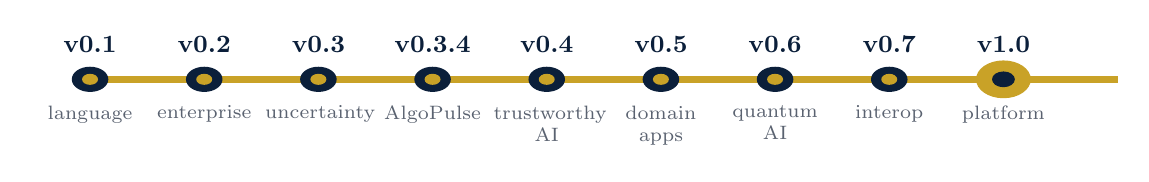
\begin{tikzpicture}[x=1.45cm]
\draw[gold,line width=2.5pt] (0,0) -- (9,0);
\foreach \x/\v/\t in {0/v0.1/language,1/v0.2/enterprise,2/v0.3/uncertainty,3/v0.3.4/AlgoPulse,4/v0.4/trustworthy AI,
  5/v0.5/domain apps,6/v0.6/quantum AI,7/v0.7/interop,8/v1.0/platform} {
  \fill[navy] (\x,0) circle (0.16); \fill[gold] (\x,0) circle (0.07);
  \node[above=6pt,font=\small\bfseries,text=navy] at (\x,0) {\v};
  \node[below=6pt,font=\scriptsize,text=muted,text width=1.35cm,align=center] at (\x,0) {\t};}
\fill[gold] (8,0) circle (0.24); \fill[navy] (8,0) circle (0.1);
\end{tikzpicture}

\vspace{14pt}
\begin{columns}[T]
\column{0.48\textwidth}\goldbox{6cm}{\small\textbf{\color{navy}Latest: 1.0} typed messages · AlgoIR and AlgoVM · signed packages · Studio SSO and roles.}
\column{0.48\textwidth}\navybox{6cm}{\small\textbf{\textcolor{gold}{After 1.0}} AlgoVM for browser and edge · organisation registries · federated review · long-running agents.}
\end{columns}
\end{frame}

% ═════════════════════════════ 22 · Getting started ═════════════════════════════
\begin{frame}[fragile]{Getting started in five minutes}
\begin{columns}[T]
\column{0.5\textwidth}
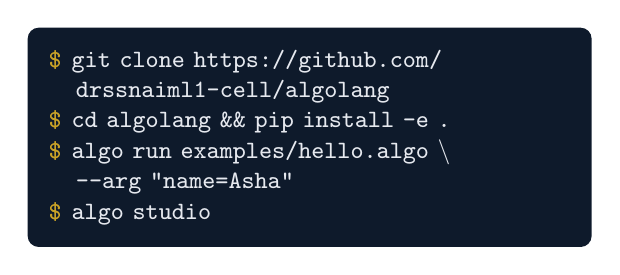
\begin{tikzpicture}
\node[fill=termbg,rounded corners=4pt,inner sep=8pt,text width=6.6cm,font=\ttfamily\small,text=termfg,align=left]{
\textcolor{gold}{\$} git clone https://github.com/\\\quad drssnaiml1-cell/algolang\\
\textcolor{gold}{\$} cd algolang \&\& pip install -e .\\
\textcolor{gold}{\$} algo run examples/hello.algo \textbackslash\\\quad --arg "name=Asha"\\
\textcolor{gold}{\$} algo studio};
\end{tikzpicture}
\vspace{4pt}

\small Runs offline with the mock model; add \texttt{ANTHROPIC\_API\_KEY} and \texttt{--live} for real models.
\column{0.47\textwidth}
\begin{itemize}\setlength\itemsep{4pt}\small
\item \textbf{50 sample programs} with a PDF guide.
\item \textbf{108-page language manual} (PDF).
\item \textbf{Website}: playground and package registry.
\item \textbf{Releases} with wheels for every version.
\end{itemize}
\end{columns}
\end{frame}

% ═════════════════════════════ 23 · Collaborate ═════════════════════════════
\begin{frame}{Collaborate with us}
\begin{columns}[T]
\column{0.5\textwidth}
\begin{itemize}\setlength\itemsep{6pt}
\item \textbf{Researchers and Ph.D.\ scholars}: agentic AI, XAI, AI governance, quantum AI; joint papers and theses.
\item \textbf{Universities}: teach governed AI with a language built for it.
\item \textbf{Industry}: pilot trustworthy agents in a real workflow.
\item \textbf{Developers}: contribute to an open-source language.
\end{itemize}
\column{0.47\textwidth}
\goldbox{5.9cm}{\textbf{\color{navy}Open research questions}\\[3pt]\small
\textcolor{gold}{■} Fairness guarantees at compile time\\
\textcolor{gold}{■} Verifying quantum answers before agents act\\
\textcolor{gold}{■} Auditable AI decisions in health and finance\\
\textcolor{gold}{■} Typed messages and multi-agent reliability}
\end{columns}
\end{frame}

% ═════════════════════════════ Build with us ═════════════════════════════
\begin{frame}{Build your application with AlgoLang}{Governed AI for your sector, from pilot to production}
\begin{columns}[T]
\column{0.5\textwidth}
\begin{itemize}\setlength\itemsep{7pt}
\item \textbf{Pilot}: a governed agent in one of your real workflows, with evals and an evidence pack.
\item \textbf{Custom applications}: a sector application like the 22 shown here, built on your tools and policies.
\item \textbf{Training}: teach teams and students to build and audit trustworthy agents.
\item \textbf{Research}: joint papers and theses on agentic AI, XAI, AI governance and quantum AI.
\end{itemize}
\column{0.47\textwidth}
\navybox{6.4cm}{\large\bfseries Applications \& partnerships\\[6pt]
{\Large\href{mailto:cto@algoprofessor.com}{\textcolor{gold}{cto@algoprofessor.com}}}\\[10pt]
\small\mdseries\color{navylight}Leadership\enspace\textcolor{white}{ceo@algoprofessor.com}\\[2pt]
Web\enspace\textcolor{white}{www.algoprofessor.com}\\[2pt]
Code\enspace\textcolor{white}{github.com/drssnaiml1-cell/algolang}\\[6pt]
\footnotesize AlgoProfessor AI R\&D Solutions, Hyderabad, India}
\end{columns}
\end{frame}

% ═════════════════════════════ 24 · Thank you ═════════════════════════════
{\setbeamertemplate{footline}{}
\begin{frame}[plain]
\begin{tikzpicture}[remember picture,overlay]
  \fill[navy] (current page.south west) rectangle (current page.north east);
  \fill[gold] ([yshift=1.6cm]current page.south west) rectangle ([yshift=1.68cm]current page.south east);
  \node[text=white,font=\fontsize{40}{44}\selectfont\bfseries] at ([yshift=1.7cm]current page.center) {Thank \textcolor{gold}{you}};
  \node[text=white,font=\large] at ([yshift=0.6cm]current page.center) {Build AI people can trust, then prove it.};
  \node[text=white,font=\large\bfseries] at ([yshift=-0.6cm]current page.center) {Dr.\ S.\ Satyanarayana, Ph.D., PDF (AI)};
  \node[text=navylight,font=\small] at ([yshift=-1.15cm]current page.center)
    {Founder, CEO \& Chief Agentic AI Scientist · AlgoProfessor AI R\&D Solutions, Hyderabad};
  \node[text=gold,font=\small\ttfamily] at ([yshift=-1.75cm]current page.center)
    {Applications: cto@algoprofessor.com \quad·\quad github.com/drssnaiml1-cell/algolang};
  \node[text=navylight,font=\scriptsize] at ([yshift=0.8cm]current page.south) {AlgoLang is open source under the Apache 2.0 licence.};
\end{tikzpicture}
\end{frame}}

\end{document}
